
\documentclass[letterpaper, reqno,11pt]{article}
\usepackage[margin=1.0in]{geometry}
\usepackage{color,latexsym,amsmath,amssymb}
\usepackage{fancyhdr}
\usepackage{amsthm}
\usepackage{mathtools}
\usepackage{tikz}
\usepackage{float}
\usepackage{centernot}
\usepackage{subcaption}
\usepackage{extarrows}
\usetikzlibrary{hobby}
\usetikzlibrary{shapes.multipart}
\usepackage{pgfplots}
\pgfplotsset{compat=1.7}
\usetikzlibrary{arrows.meta}
\usepackage{cancel}
\usetikzlibrary{decorations.markings}
\usetikzlibrary{shapes}

\newcommand{\RR}{\mathbb{R}}
\newcommand{\CC}{\mathbb{C}}
\newcommand{\ZZ}{\mathbb{Z}}
\newcommand{\QQ}{\mathbb{Q}}
\newcommand{\NN}{\mathbb{N}}
\def\upint{\mathchoice%
  {\mkern13mu\overline{\vphantom{\intop}\mkern7mu}\mkern-20mu}%
  {\mkern7mu\overline{\vphantom{\intop}\mkern7mu}\mkern-14mu}%
  {\mkern7mu\overline{\vphantom{\intop}\mkern7mu}\mkern-14mu}%
  {\mkern7mu\overline{\vphantom{\intop}\mkern7mu}\mkern-14mu}%
  \int}
\def\lowint{\mkern3mu\underline{\vphantom{\intop}\mkern7mu}\mkern-10mu\int}
\DeclareMathOperator{\card}{card}
\DeclareMathOperator{\Binomial}{Binomial}
\DeclareMathOperator{\Span}{span}
\pagestyle{fancy}
\lhead{Math 321 Lecture 24}
\rhead{Yuchong Pan}
\begin{document}
\pagenumbering{arabic}
\title{Math 321 Lecture 24}
\author{Yuchong Pan}
\date{March 6, 2019}
\newtheorem{thm}{Theorem}
\newtheorem{defn}{Definition}
\newtheorem*{remark}{Remark}
\newtheorem{claim}{Claim}
\newtheorem{cor}{Corollary}
\newtheorem{lemma}{Lemma}
\newtheorem{prop}{Proposition}
\newtheorem{fact}{Fact}
\maketitle
%

\section{Fourier Series (Cont'd)}

\subsection{Inner Product Spaces}

\begin{defn}
  \normalfont Let $V$ be a vector space over $\CC$ (or $\RR$). Say $\langle \cdot, \cdot \rangle : V \times V \to \CC \text{ or $\RR$}$ is an {\bf inner product} if it obeys the following properties:
  \begin{enumerate}
  \item Conjugate symmetry: $\langle \mathbf v, \mathbf w \rangle = \overline{\langle \mathbf w, \mathbf v \rangle}$ for all $\mathbf v, \mathbf w \in V$.
  \item Linearity in the first coordinate:
    \begin{align*}
      \langle \alpha \mathbf v, \mathbf w \rangle &= \alpha \langle \mathbf v, \mathbf w \rangle, && \forall \alpha \in \CC, \mathbf v, \mathbf w \in V, \\
      \langle \mathbf v_1 + \mathbf v_2, \mathbf w \rangle &= \langle \mathbf v_1, \mathbf w \rangle + \langle \mathbf v_2, \mathbf w \rangle, && \forall \mathbf v_1, \mathbf v_2, \mathbf w \in V. \\
    \end{align*}
  \item Positive definiteness: For any $\mathbf v \in V$, $\langle \mathbf v, \mathbf v \rangle$ is a non-negative real number. $\langle \mathbf v, \mathbf v \rangle = 0$ if and only if $\mathbf v = \mathbf 0$.
  \end{enumerate}
\end{defn}

\noindent {\bf Examples:}
\begin{enumerate}
\item $\RR^n$ or $\CC^n$. Let $\mathbf v = (v_1, \ldots, v_n)$ and $\mathbf w = (w_1, \ldots, w_n)$. Then,
  \[ \langle \mathbf v, \mathbf w \rangle = \sum_{j = 1}^n v_j \overline{w_j} = \text{Euclidean dot product of $\mathbf v$ and $\mathbf w$}. \]
\item $\ell^2(\NN) = \left\{ \mathbf x = (x_1, x_2, x_3, \ldots) : x_j \in \CC, \sum_{j = 1}^\infty |x_j|^2 < \infty \right\}$. Define
  \[ \langle \mathbf x, \mathbf y \rangle = \sum_{j = 1}^\infty x_j \overline{y_j}. \]
  This is well-defined as an absolutely convergent infinite series because
  \[ \sum_{j = 1}^n \left\lVert x_j \overline{y_j} \right\rVert \underbrace{\leq}_\text{Cauchy-Schwarz} \left(\sum_{j = 1}^n |x_j|^2\right)^\frac{1}{2} \left(\sum_{j = 1}^n |y_j|^2\right)^\frac{1}{2}, \]
  and let $n \to \infty$.
\item $L_*^2[-\pi, \pi] = \mathcal C^{2\pi}$, equipped with the norm
  \[ \lVert f \rVert_2 = \left[\frac{1}{2\pi} \int_{-\pi}^\pi |f(x)|^2 dx\right]^\frac{1}{2}. \]
  (Aside: $L^2[0, 1] = \left\{ f : \int_0^1 |f(x)|^2 dx < \infty \right\}$.)
  Define
  \[ \langle f, g \rangle = \frac{1}{2\pi} \int_{-\pi}^\pi f(x) \overline{g(x)} dx. \]
\end{enumerate}

\begin{figure}[H]
  \centering
  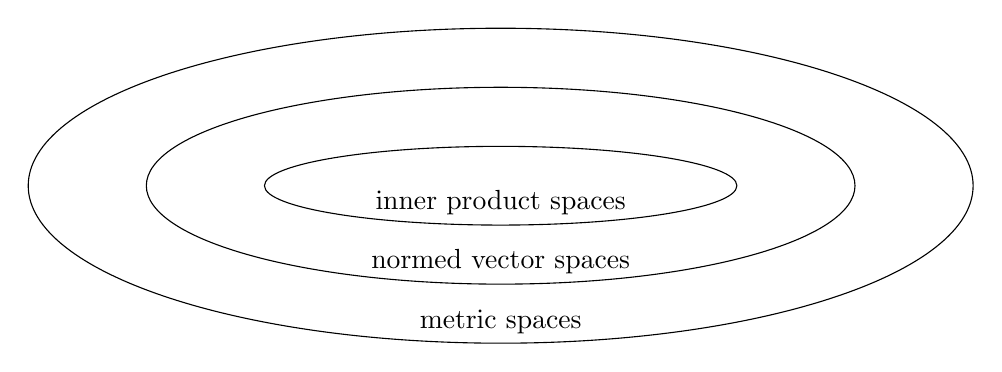
\begin{tikzpicture}
    \draw (0, 0) ellipse (6 and 2);
    \node[above] at (0, -2) {metric spaces};
    \draw (0, 0) ellipse (4.5 and 1.25);
    \node[above] at (0, -1.25) {normed vector spaces};
    \draw (0, 0) ellipse (3 and 0.5);
    \node[above] at (0, -0.5) {inner product spaces};
  \end{tikzpicture}
\end{figure}

\noindent {\bf Facts:}
\begin{enumerate}
\item Every inner product generates a norm on $V$; $\lVert \mathbf v \rVert = \sqrt{\langle \mathbf v, \mathbf v \rangle}$. Check that this obeys the properties of a norm.
\item \label{enum:2} Every inner product obeys the Cauchy-Swartz inequality
  \[ |\langle \mathbf v, \mathbf w \rangle| \leq \lVert \mathbf v \rVert \cdot \lVert \mathbf w \rVert. \qquad \text{(Exercise)} \]
\item Note that \ref{enum:2} offers a way to define the notion of ``angle'' between two vectors $\mathbf v$ and $\mathbf w$; we say that the angle between $\mathbf v$ and $\mathbf w$ is $\theta$ if
  \[ \cos\theta = \frac{|\langle \mathbf v, \mathbf w \rangle|}{\lVert \mathbf v \rVert \cdot \lVert \mathbf w \rVert}. \]

  \begin{figure}[H]
    \centering
    \begin{tikzpicture}
      \draw (0, 0) -- (10, 0);
      \draw (8, 4) -- (2, 0) node[below] {$\mathbf 0$};
      \draw (8, 4) -- (8, 0) node[below] {$\mathbf w$};
      \node[above] at (8, 4) {$\mathbf v$};
      \draw (7.75, 0) |- (8, 0.25);
    \end{tikzpicture}
  \end{figure}
\item Many identities from Eucliean geometry carry over to an inner product space $V$.
  \begin{enumerate}
  \item {\bf Pythagorean theorem:} Suppose $\mathbf v, \mathbf w \in V$ with $\mathbf v \perp \mathbf w$ (i.e., $\langle \mathbf v, \mathbf w \rangle = 0$). Then,
    \[ \lVert \mathbf v + \mathbf w \rVert^2 = \lVert \mathbf v \rVert^2 + \lVert \mathbf w \rVert^2. \]
    
    \begin{figure}[H]
      \centering
      \begin{tikzpicture}
        \draw (0, 0) -- (6, 4) node[midway, above left] {$\mathbf v + \mathbf w$};
        \draw[decoration={
            markings,
            mark=at position 0.5 with {\arrow{>}}},
          postaction={decorate}
        ] (0, 0) -- (6, 0) node[midway, below] {$\mathbf v$};
        \draw[decoration={
            markings,
            mark=at position 0.5 with {\arrow{>}}},
          postaction={decorate}
        ] (6, 0) -- (6, 4) node[midway, right] {$\mathbf w$};
      \end{tikzpicture}
    \end{figure}
  \item {\bf Parallelogram law:}
    \[ \lVert \mathbf x + \mathbf y \rVert^2 + \lVert \mathbf x - \mathbf y \rVert^2 = 2 \left[ \lVert \mathbf x \rVert + \lVert \mathbf y \rVert^2 \right], \]
    for all $\mathbf x, \mathbf y$ in an inner product space.

    \begin{figure}[H]
      \centering
      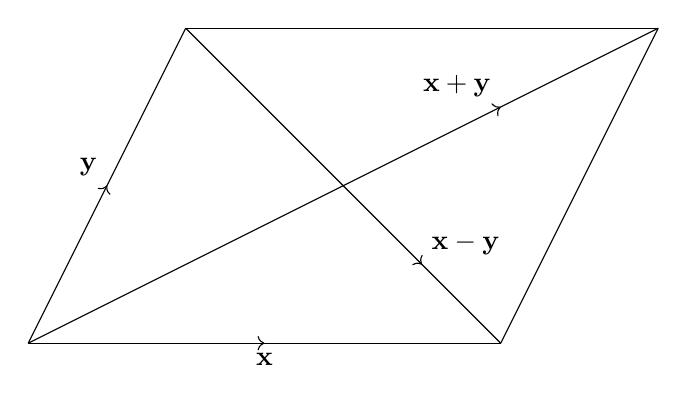
\begin{tikzpicture}
        \draw[decoration={
            markings,
            mark=at position 0.5 with {\arrow{>}}},
          postaction={decorate}
        ] (0, 0) -- (6, 0) node[midway, below] {$\mathbf x$};
        \draw[decoration={
            markings,
            mark=at position 0.5 with {\arrow{>}}},
          postaction={decorate}
        ] (0, 0) -- (2, 4) node[midway, above left] {$\mathbf y$};
        \draw (2, 4) -- (8, 4);
        \draw (6, 0) -- (8, 4);
        \draw (0, 0) -- (8, 4)[decoration={
            markings,
            mark=at position 0.75 with {\arrow{>}}},
          postaction={decorate}
        ] node[above left, pos=0.75] {$\mathbf x + \mathbf y$};
        \draw (2, 4) -- (6, 0)[decoration={
            markings,
            mark=at position 0.75 with {\arrow{>}}},
          postaction={decorate}
        ] node[above right, pos=0.75] {$\mathbf x - \mathbf y$};
      \end{tikzpicture}
    \end{figure}

    \noindent {\bf Exercise:} Use the parallelogram law to show that if $\ell^p$ or $L_*^p$ is an inner product space, then $p = 2$.
  \end{enumerate}
\end{enumerate}

\subsection{Uniform Convergence (or Lackthereof) of Fourier Series}

\noindent {\bf Message:}
\begin{enumerate}
\item If $f$ is merely known to be continuous and $2\pi$-periodic, then it is \emph{not} in general true that \fbox{$S_n f \xrightarrow{n \to \infty} f$ uniformly} (i.e., $\sup_{x \in [-\pi, \pi]} |s_n f(x) - f(x)| = \lVert s_n f - f \rVert_\infty \xrightarrow{n \to \infty} 0$) or even pointwise.
\item Plancherel: $\lVert s_n f - f \rVert_2 \xrightarrow{n \to \infty} 0$.
\end{enumerate}

\begin{align*}
  & \underbrace{\text{\bf uniform convergence}}_{\substack{\text{$f_n \to f$ uniformly} \;\Leftrightarrow\; \\ \sup_x |f_n(x) - f(x)| \xrightarrow{n \to \infty} 0}} \Rightarrow \underbrace{\text{\bf pointwise convergence}}_\text{For every $x$, $f_n(x) \xrightarrow{n \to \infty} f(x)$}, \\
  & \text{\bf $L^2$ convergence: $\int_{-\pi}^\pi |f_n(x) - f(x)|^2 \to 0$}.
\end{align*}

\end{document}
